%************************************************
\chapter{Abstract Probabilistic Rewriting}\label{ch:mathtest} % $\mathbb{ZNR}$
%************************************************
The $\lambda$-calculus is essentially a rewrite system. Thus, before introducing it, we present some fundamentals of rewriting theory. This way we can insert the $\lambda$-calculus into a more general setting, allowing a deeper and often simpler analysis. Rewriting is crucial in computer science: basically any computation can be seen as a process of rewriting. In fact, digital computers work through formal manipulation of symbols, in a purely syntactic way. Rewriting theory was born together with logic, but now it has an independent status, as shown by the annual International Conference on Rewriting Techniques and Applications (RTA) \cite{noauthor_rta_nodate}, now part of the International Conference on Formal Structures for Computation and Deduction along with the  International Conference on Typed Lambda Calculi and Applications \cite{noauthor_notitle_nodate}, just to remark the strong connection between the two fields.
\section{Abstract Rewriting Theory}
The basic object of investigation of rewriting theory is the abstract reduction (or rewrite) system. 
\begin{definition}
	An \emph{abstract reduction system} (ARS) is a pair $(A,\rightarrow)$ where $A$ is a set with cardinality at most countable and $\rightarrow\,\subseteq A\times A$.
\end{definition}
$A$ is the set of \emph{terms} and $\rightarrow$ is the \emph{reduction relation}. If $(a,b)\in\,\rightarrow$ for $a,b\in A$, we write $a\rightarrow b$ and intuitively this means that ``$a$ can be rewritten in $b$''. An important characteristic of ARSs is that $\red$ is not in general a (partial) function. This means that a term can be rewritten to more than one term, i.e. the rewriting process is not deterministic. We call an ARS $(A,\rightarrow)$ \emph{deterministic} (DARS) if $\red$ is a partial function. $\twoheadrightarrow$ is the reflexive and transitive closure of $\rightarrow$. A \emph{reduction sequence} is a finite or infinite sequence $\sigma:a_0\rightarrow a_1\rightarrow\cdots$. If $\sigma$ is finite, then $|\sigma|$ is the \emph{length} of $\sigma$. Since rewriting is a model of computation, we are interested in defining termination. We say that $a\in A$ is in \emph{normal form} if there exist no $b\in A$ such that $a\rightarrow b$. We call $\mathbf{NF}(A)$ the set of terms in normal form of $A$. A term $a$ is \emph{(weakly) normalising} if there exists a reduction sequence such that $a\twoheadrightarrow b$ and $b$ is in normal form. A term $a$ is \emph{strongly normalising} if every reduction sequence from $a$ is finite.  A lot of interesting properties can be defined for ARSs. The interested reader can refer to the two main monographs on the subject \cite{terese_term_2003,baader_term_1999} for a complete account on them. However, it is worth mentioning here a very important property, namely confluence.
\begin{definition}
	Let $(A,\rightarrow)$ be an ARS. $\rightarrow$ is \emph{confluent} or \emph{Church-Rosser} (CR), if for each $a\in A$ such that $a\twoheadrightarrow b$ and $a\twoheadrightarrow c$, there exists $d\in A$ such that $b\twoheadrightarrow d$ and $c\twoheadrightarrow d$.
\end{definition}
Confluence is a desirable property because intuitively it states that no matter the reduction path followed, one can always reconcile those paths, possibly going further with the reductions (Figure \ref{figure:confluence}). In particular confluence is sufficient for an ARS to satisfy the unique normal form property, we are defining below.
\begin{figure}
	\fbox{
		\begin{minipage}{.96\textwidth}
	\centering
	\subfloat[]{{	
			\begin{tikzpicture}
			[node distance=20mm, auto, transform shape]
			\node (m) at (0,0) {$a$};
			\node (n) at (-1,-1) {$b$};
			\node (l) at (1,-1) {$c$};
			\draw (m) edge[->>] node[left=5pt] {} (n);
			\draw (m) edge[->>] node[right=5pt] {} (l);
			\end{tikzpicture}}}
	\qquad
	\subfloat[]{{	
			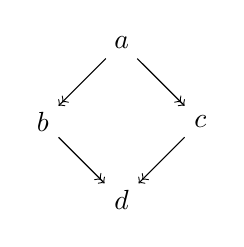
\begin{tikzpicture}
			[node distance=20mm, auto, transform shape]
			\node (m) at (0,0) {$a$};
			\node (n) at (-1,-1) {$b$};
			\node (l) at (1,-1) {$c$};
			\node (p) at (0,-2) {$d$};
			\draw (m) edge[->>] node[left=5pt] {} (n);
			\draw (m) edge[->>] node[right=5pt] {} (l);
			\draw (n) edge[->>] node[left=5pt] {} (p);
			\draw (l) edge[->>] node[right=5pt] {} (p);
			\end{tikzpicture}}}
	\end{minipage}}
	\caption{CR holds if (a) implies (b)}
	\label{figure:confluence}
\end{figure}
\begin{definition}
	Let $(A,\rightarrow)$ be an ARS. $\rightarrow$ has the \emph{unique normal form property} (UN) if for each $a,b,c\in A$, such that $a\twoheadrightarrow b$, $a\twoheadrightarrow c$, and $b,c\in\mathbf{NF}(A)$, then $b= c$.
\end{definition}
Uniqueness of normal form is a key aspect when we are dealing with ARSs. In fact, typically, we want that a given term always terminates in the same result, although possibly following different paths.
\begin{proposition}
	Let $(A,\rightarrow)$ be an ARS. If $\rightarrow$ is confluent then $\rightarrow$ has the unique normal form property.
\end{proposition}
\begin{proof}
	By contradiction, let us consider an ARS $(A,\rightarrow)$ such that $\rightarrow$ is confluent but does not satisfy UN. Then there exist $a,b,c\in A$, such that $a\twoheadrightarrow b$, $a\twoheadrightarrow c$, $b,c\in\mathbf{NF}(A)$ and $b\not\equiv c$. Since $\rightarrow$ is confluent, there exists $d\in A$ such that $b\twoheadrightarrow d$ and $c\twoheadrightarrow d$. Since both $b$ and $c$ are in normal form this would imply $d\equiv b\equiv c$ but this is impossible since $b$ and $c$ are different normal forms.
\end{proof}
ARSs are sets endowed with a relation, and are thus
inherently nondeterministic, if we consider rewriting as a model of a computation. The notion of reduction strategy allows us to turn reduction into a deterministic process.
\begin{definition}[Deterministic Strategies]\label{def:determstrat}
	Given an ARS $(A,\rightarrow)$, a \emph{deterministic reduction
		strategy for $A$} is a partial function $\mathsf{S}:A\rightharpoonup A$
	such that $\mathsf{S}(a)$ is defined if and only if $a$ is not in
	normal form and $a\rightarrow\mathsf{S}(a)$ whenever $\mathsf{S}(a)$
	is defined.
	%$\mathsf{S}(a)\in\{b\,|\,a\rightarrow b\}$.
\end{definition}
\begin{definition}
	A reduction sequence $\sigma:a_0\rightarrow a_1\rightarrow\cdots\rightarrow a_n$ is \emph{under strategy} $\mathsf{S}$ if $\mathsf{S}(a_i)=a_{i+1}$ for each $0\leq i<n$.
\end{definition}
If $\sigma:a_0\rightarrow a_1\rightarrow\cdots\rightarrow a_n$ is a
reduction sequence under strategy $\mathsf{S}$ and $a_n$ is in normal
form, we write $\nsteps{\mathsf{S}}(a_0)=n=|\sigma|$. If
$\sigma:a_0\rightarrow a_1\rightarrow\cdots$ is infinite, we say that
$\nsteps{\mathsf{S}}(a_0)=+\infty$. A strategy $\mathsf{S}$ is \emph{normalising} if for each weakly normalising term $a$, $\nsteps{\mathsf{S}}(a)<+\infty$. Reductions to normal form of the same term under different strategies can be of different lengths, and in particular some of them can be infinite. However, under particular conditions, all strategies are equivalent.
\begin{definition}
	An ARS $(A,\red)$ satisfies the \emph{(weak) diamond property} (WDP) if and only if for each term $a\in A$, if $a\red b$ and $a\red c$, then either $b=c$ or there exists a term $d\in A$ such that $b\red d$ and $c\red d$. 
\end{definition}
Intuitively an ARS satisfies the WDP if we can close every diagram in \emph{just one} step, forming a diamond (Figure \ref{figure:diam}). This very strong property is sufficient to state that all reduction sequences from a term to its normal form have the \emph{same} length, i.e. no matter the strategy chosen to select the reduct.
\begin{figure}
	\fbox{
		\begin{minipage}{.96\textwidth}
	\centering
	\subfloat[]{{	
			\begin{tikzpicture}
			[node distance=20mm, auto, transform shape]
			\node (m) at (0,0) {$a$};
			\node (n) at (-1,-1) {$b$};
			\node (l) at (1,-1) {$c$};
			\node (eq) at (0,-1) {$\neq$};
			\draw (m) edge[->] node[left=5pt] {} (n);
			\draw (m) edge[->] node[right=5pt] {} (l);
			\end{tikzpicture}}}
	\qquad
	\subfloat[]{{	
			\begin{tikzpicture}
			[node distance=20mm, auto, transform shape]
			\node (m) at (0,0) {$a$};
			\node (n) at (-1,-1) {$b$};
			\node (l) at (1,-1) {$c$};
			\node (p) at (0,-2) {$d$};
			\draw (m) edge[->] node[left=5pt] {} (n);
			\draw (m) edge[->] node[right=5pt] {} (l);
			\draw (n) edge[->] node[left=5pt] {} (p);
			\draw (l) edge[->] node[right=5pt] {} (p);
			\end{tikzpicture}}}
	\end{minipage}}
	\caption{WDP holds if (a) implies (b)}
	\label{figure:diam}
\end{figure}
\begin{lemma}[]\label{lemma:weak}
	If an ARS $(A,\red)$ satisfies the weak diamond property, then for each term $a\in A$ that has a normal form, all reduction sequences from $a$ to its normal form have the same length.
\end{lemma}
\begin{proof}
	The proof by induction is given with all details in \cite{dal_lago_invariant_2005}.
\end{proof}
\section{Probabilistic Rewriting}
As we have already pointed out, rewriting theory is now a well-established field of theoretical computer science. Methods from this area have been applied to a variety of problems, such as program transformation and optimisation and formal verification of protocols. Traditionally, rewriting is a nondeterministic model and strategies are the technical tool that allows a deterministic rewriting. However, in recent years, more and more attention has been given to \emph{probabilistic computation}. Actually stochastic models and computer science are linked from the early days of both these disciplines. Already in 1963, Micheal Rabin proposed his model of probabilistic automata \cite{rabin_probabilistic_1963} and in the seventies the first examples of randomised algorithms were given again by Rabin, e.g.the Miller-Rabin primality test \cite{rabin_probabilistic_1980}. Later, in the eighties, cryptography acquired the status of formal science through the use of probability theory \cite{goldreich_how_1984}. Nowadays machine learning is one of the main tools used in artificial intelligence and it is very rooted in statistics and stochastic inference methods. Programming language community was thus challenged to create easy, flexible and powerful \emph{probabilistic programming languages} with primitive operators such us the \emph{sample} from a distribution \cite{goodman_church:_2008,wood_new_2014}. However, the study of their semantics is not trivial \cite{staton_semantics_2016}, and even the definition of termination is not obvious in a probabilistic setting. Probabilistic rewriting is one of the tools developed to model  probabilistic functional programming languages \cite{avanzini_probabilistic_2018}. However, our work exploits probabilistic rewriting in a different and novel sense, in the realm of the $\lambda$-calculus. In fact our calculus remains deterministic, in that there is not a \emph{choice} operator like in \cite{borgstrom_lambda-calculus_2016}. What becomes stochastic is the choice of the redex to reduce, namely the strategy. Strategies this way map terms to \emph{distributions} on terms. We start defining probabilistic abstract rewriting, while in Chapter~\ref{chapter:prostra} we analyse the $\lambda$-calculus equipped with randomised strategies.
\subsection{Probabilistic Abstract Reduction Systems as Strategies}
We introduce now the framework we are going to define randomised
strategies within. In particular, we shift the notion of ARS to the fully
probabilistic case. With respect to standard Markov chain theory, our
construction is simpler and allows to reason better in an infinite
state context. The first preliminary concept we need is that of a distribution.
\begin{definition}[Distribution]
	A \emph{partial probability distribution} over a countable set $A$
	is a mapping $\rho:A\rightarrow\left[0,1\right]$ such that
	$\left|\rho\right|\leq 1$ where
	$\left|\rho\right|=\underset{a\in A}{\sum}\rho\left(a\right)$. We denote the set of partial probability distributions over $A$
	by $\pdist{A}$. The \emph{support} of a partial distribution
	$\rho\in\pdist{A}$ is the set $\supp{\rho}=\left\lbrace a \in A \, |
	\, \rho\left( a\right) >0\right\rbrace $.  A \emph{probability
		distribution} over a countable set $A$ is a partial probability
	distribution $\mu$ such that $\left|\mu\right|=1$. $\dist{A}$ denotes the set
	of probability distributions over $A$.
\end{definition}
Sometimes we have to deal with \emph{deterministic} distributions. This can be done considering a distribution $\mu$ such that $|\supp{\mu}|=1$.
\begin{definition}
	A distribution $\mu\in\dist{S}$ is $\textbf{Dirac}$ if there exists $s\in S$ such that $\mu(s)=1$. In this case we write $\mu=\textbf{Dirac}(s)$.
\end{definition}
Strategies as from Definition~\ref{def:determstrat} are inherently
deterministic: the process of picking a reduct among the many possible
ones can only have \emph{one} outcome. But what if this process becomes
\emph{probabilistic}? This is captured by the following notion:
\begin{definition}[Randomised Strategies]
	Given an ARS $(S,\rightarrow)$, a
	\emph{randomised reduction strategy $\mathsf{P}$ for $(S,\rightarrow)$}
	is a partial function such that if $s\in S$ is in normal form, then
	$\mathsf{P}(s)=\bot$, otherwise $\mathsf{P}(s)=\mu\in\dist{S}$, and
	$\supp{\mu}\subseteq\{t\,|\,s\rightarrow t\}$.
	%\emph{fully probabilistic abstract
	%  reduction system (FPARS) for $(S,\rightarrow)$} is a pair $\left(
	%S,\mathsf{P}\right)$ where $\mathsf{P}:S\rightharpoonup\dist{S}$ is
	% We call $\mathsf{P}$
	%a \emph{randomised reduction strategy for $(S,\rightarrow)$}.
\end{definition}
Please notice that if $(S,\rightarrow)$ is an ARS and 
$\mathsf{P}$ is a randomised reduction strategy for it,
then $(S,\mathsf{P})$ can be seen as a \emph{fully} probabilistic abstract
reduction system (FPARS), namely a probabilistic abstract reduction
system~\cite{avanzini_probabilistic_2018} whose dynamics is purely
probabilistic, without any nondeterminism. In the following, we will
study randomised strategies as FPARS.

The dynamics of an FPARS can be handled by way of an appropriate
notion of a configuration, on which an evolution function can be
defined:
\begin{definition}[Configurations, Computations]
	Let $\left( S,\mathsf{P}\right)$ be an FPARS and $s,t\in S$ be two
	\emph{states}. We define the probability $\mathbb{P}\left(s
	\rightarrow t\right)$ of a \emph{transition} from $s$ to $t$:
	$$
	\mathbb{P}\left(s \rightarrow t\right)=
	\begin{cases}
	\mu\left(t\right)&\mbox{if $\mathsf{P}\left(s\right)=\mu$},\\
	0&\mbox{if $\mathsf{P}\left(s\right)=\bot$}.
	\end{cases}
	$$
	A \emph{configuration} of an FPARS $\left( S,\mathsf{P}\right)$ is a partial probability distribution $\rho\in\pdist{S}$.
	The \emph{evolution} of an FPARS $\left( S,\mathsf{P}\right)$ from a configuration $\rho$ is a function $\mathsf{E}:\pdist{S}{\rightarrow\pdist{S}}$ defined in the following way:
	$$
	\mathsf{E}\left( \rho\right) = \sigma \textnormal{ where } \sigma\left(s\right)=\underset{t\in S}{\sum}\rho\left( t\right) \cdot\mathbb{P}\left(t \rightarrow s\right)\;\textnormal{for every }s \in S.
	$$
	If  $\mathsf{E}\left( \rho\right) = \sigma$ we write $\rho\rightsquigarrow\sigma$.
	A \emph{computation} is any sequence
	$(\rho_i)_{i\in\mathbb{N}}$, such that $\rho_i\rightsquigarrow\rho_{i+1}$.
\end{definition}
\begin{remark}
	Those computations $(\rho_i)_{i\in\mathbb{N}}$ where
	$\rho_0$ is $\mathbf{Dirac}$ (i.e. there exists $s\in S$ such that
	$\rho_0 (s)=1$) are particularly interesting: they model
	the evolution of an FPARS starting from one state. We write in this case
	$\rho_0=\mathbf{Dirac}(s)$.
\end{remark}
\begin{example}\label{example:pars}
	Consider an ARS $(S,\rightarrow)$, where $S=\{a,b\}$ and $\rightarrow\,=\{(a,a),(a,b)\}$. We define a randomised strategy $\mathsf{P}$ on top of $(S,\rightarrow)$. $\mathsf{P}(a)=\mu$ such that $\mu(a)=\mu(b)=\frac{1}{2}$, while $\mathsf{P}(b)=\bot$ since $b$ is in normal form. A computation $(\rho_i)_{i\in\mathbb{N}}$ starting from $\rho_0=\mathbf{Dirac}(a)$ has the following form.
	$$
	\underset{\rho_{0}}{\begin{cases}
		1 & a\\
		0 & b
		\end{cases}}\rightsquigarrow\underset{\rho_{1}}{\begin{cases}
		\frac{1}{2} & a\\
		\frac{1}{2} & b
		\end{cases}}\rightsquigarrow\underset{\rho_{2}}{\begin{cases}
		\frac{1}{4} & a\\
		\frac{1}{4} & b
		\end{cases}}\rightsquigarrow\cdots\rightsquigarrow\underset{\rho_{k}}{\begin{cases}
		\frac{1}{2^{k}} & a\\
		\frac{1}{2^{k}} & b
		\end{cases}}\rightsquigarrow\cdots
	$$
\end{example}
How could we measure the \emph{length} of a computation starting from $s$? Since the setting is probabilistic, it is natural
to look for a definition capturing the \emph{average} derivation length from
$s$ to its normal form. 
\begin{definition}
	Let $(S,\mathsf{P})$ be an FPARS and $\rho_0=\mathbf{Dirac}(s)$,
	where $s\in S$. Given the computation $(\rho_i)_{i\in\mathbb{N}}$,
	$\nsteps{\mathsf{P}}(s)=\sum\limits_{i=1}^{\infty} \left|\rho_i\right|$.
\end{definition}
In the next section we will show that $\nsteps{}$ is actually the expected value of a properly defined random variable. Observe that the definition above collapses to the one given for the
deterministic case when $\mathsf{P}$ is deterministic. 
\begin{SHORT}
	That it is the expected value of a random variable capturing the number of reduction
	steps to normal form from $s$ can be proved by standard arguments
	from the theory of Markov Chains, see~\cite{EV} for details.
\end{SHORT}
Termination is a crucial problem in rewriting theory. Since we are in
a probabilistic context, distinct such notions are
possible. We define in our setting two classical termination
properties.  
\begin{definition}
	An FPARS is \emph{almost-surely terminating} (AST) if for each initial configuration $\rho_0$, the computation $(\rho_i)_{i\in\mathbb{N}}$, is such that $\underset{n\rightarrow +\infty}{\lim}\left|\rho_{n}\right|=0$.
\end{definition}
\begin{definition}
	An FPARS $(S,\mathsf{P})$ is \emph{positive almost-surely terminating} (PAST) if for each $s \in S$,
	$\nsteps{\mathsf{P}}(s)< +\infty$.
	In this case we say that $\mathsf{P}$ is a \emph{positive almost-surely normalising} strategy.
\end{definition}
\begin{example}
	Consider the same setting of Example \ref{example:pars}. It is easy to see that $(S,\mathsf{P})$ is AST since $\underset{n\rightarrow +\infty}{\lim}\left|\rho_{n}\right|=\underset{n\rightarrow +\infty}{\lim}\frac{1}{2^{n-1}}=0$. Moreover $(S,\mathsf{P})$ is PAST since $\nsteps{\mathsf{P}}(a)=\sum\limits_{n=1}^{\infty} \left|\rho_n\right|=\sum\limits_{n=1}^{\infty}\frac{1}{2^{n-1}}=2$ and $\nsteps{\mathsf{P}}(b)=0$.
\end{example}
It is well-known from Markov chain literature that AST does not imply PAST e.g. in the symmetric random walk on $\mathbb{Z}$. We prove in our framework a classical result in Markov chain theory that gives a sufficient condition for PAST and a bound on the average number of steps to normal form.
\begin{notation}
	For $\varepsilon>0$ we write $x>_{\varepsilon}y$ if and only if $x\geq y+\varepsilon$. This order is well-founded on real numbers with a lower bound.
\end{notation}
\begin{definition}
	Given an FPARS $\left( S,\mathsf{P}\right)$, we define a function $V:S\rightarrow\mathbb{R}$ as Lyapunov if:
	\begin{varitemize}
		\item
		There exists $b\in\mathbb{R}$ such that $V\left(s\right)\geq b$ for each $s\in S$.
		\item
		There exists $\varepsilon>0$ such that for every $s\in S$ if $\mathsf{P}\left(s\right) = \mu$, then $V\left(s\right) >_{\varepsilon} V\left(\mu\right)$, where $V$ is extended to partial distributions as follows:
		$$
		V\left(\mu\right)=\sum_{t\in S}V\left(t\right)\cdot\mu\left(t\right).
		$$
	\end{varitemize}
\end{definition}
\begin{remark}
	Without loss of generality, given a Lyapunov function $V$ we can always consider a new Lyapunov function $W(s)\geq 0$ for each $s\in S$ simply adding a constant to $V$.
\end{remark}
\begin{theorem}
	If we can define for an FPARS $\mathcal{P}=\left(S,\mathsf{P}\right)$ a Lyapunov function $V$, then $\mathcal{P}$ is PAST and the average derivation length $\nsteps{\mathsf{P}}(s)$ of any sequence $(\rho_i)_{i\in\mathbb{N}}$ starting from any $s\in S$ is bounded by
	$\frac{V\left(s\right)}{\varepsilon}$.
\end{theorem}
\begin{LONG}
	\begin{proof}
		This proof partly was inspired by the one of Foster Theorem in \cite{bremaud_markov_1999}. Let us consider a generic transition $\rho_{i-1}\rightsquigarrow\rho_i$ of $\mathcal{P}$.
		\begin{equation*}
		\begin{split}
		0&\leq V(\rho_i)=\sum_{k\in S}V(k)\rho_i(k)=\sum_{k\in S}V(k)\sum_{j\in S}\rho_{i-1}(j)\cdot\delta(j\rightarrow k)\\
		&\overset{\delta(j)=\mu}{=}\sum_{k\in S}V(k)\sum_{j\in S\setminus \mathbf{NF}(S)}\rho_{i-1}(j)\cdot\mu(k)=\sum_{j\in S\setminus \mathbf{NF}(S)}\rho_{i-1}(j)\sum_{k\in S}V(k)\mu(k)\\
		&=\sum_{j\in S\setminus \mathbf{NF}(S)}\rho_{i-1}(j)\cdot V(\mu)\leq \sum_{j\in S\setminus \mathbf{NF}(S)}\rho_{i-1}(j)\cdot (V(j)-\varepsilon)\\
		&\leq \sum_{j\in S}\rho_{i-1}(j)\cdot V(j) - \sum_{j\in S\setminus \mathbf{NF}(S)}\rho_{i-1}(j)\cdot \varepsilon=V(\rho_{i-1})-\varepsilon\cdot|\rho_i|.
		\end{split}
		\end{equation*}
		Iterating the above inequality we have
		\begin{align*}
		0&\leq V(\rho_i)\leq V(\rho_{i-1})-\varepsilon\cdot|\rho_i|\leq V(\rho_{i-2})-\varepsilon\cdot(|\rho_i| + |\rho_{i-1}|)\\
		&\leq \cdots\leq V(\rho_0)-\varepsilon\cdot\sum_{n=1}^i |\rho_n|.
		\end{align*}
		Taking the limit for $n\rightarrow +\infty$ this yields to
		$$
		0\leq V(\rho_0)-\varepsilon\cdot\nsteps{\mathsf{P}}(s)
		$$
		and thus
		$$
		\nsteps{\mathsf{P}}(s)\leq \frac{V(\rho_0)}{\varepsilon}=\frac{V(s)}{\varepsilon}.
		$$
		
	\end{proof}
\end{LONG}
\begin{LONG}
	\subsection{FPARS and Markov Chains}
	We first recall some basic notions of probability theory and Markov chain theory. Please refer to \cite{ash_probability_1999,norris_markov_1998} for a more detailed discussion on the subject.
	\begin{definition}[Probability space]
		A \emph{probability space} is a triple $(\Omega, \mathcal{F},\mathbb{P})$ where $\Omega$ is the \emph{sample space}, $\mathcal{F}$ is the set of the \emph{events} and it is a $\sigma$-algebra of $\Omega$, and $\mathbb{P}$ is a \emph{probability measure} for $\mathcal{F}$ i.e. $\mathbb{P} :\mathcal{F}\rightarrow[0,1]$, $\mathbb{P}\{\Omega\}=1$ and it is countably additive: the probability of a countable disjoint union of events is given by the sum of the individual probabilities.
	\end{definition}
	\begin{definition}[Conditional probability]
		Given two events $A$ and $B$ if $\mathbb{P}\{B\}\neq 0$ the \emph{conditional probability} of $A$ given $B$ is
		$$
		\mathbb{P}\{A|B\}=\frac{\mathbb{P}\{A\cap B\}}{\mathbb{P}\{B\}}.
		$$
	\end{definition}
	\begin{definition}[Random variable]
		Let $(\Omega, \mathcal{F},\mathbb{P})$ be a probability space. A \emph{random variable} $X$ is a function from $\Omega$ to $\mathbb{R}$ such that for each $x\in \mathbb{R}$, the set $\{X\leq x\}$:=$\{\omega\in\Omega : X(\omega)\leq x\}\in \mathcal{F}$. A random variable $X$ is \emph{discrete} if there exists a set $I$ at most countable such that $\mathbb{P}\{X\in I\}=1$.
	\end{definition} 
	\begin{definition}[Expected value]
		Given a random variable $X$ on $(\Omega, \mathcal{F},\mathbb{P})$, its \emph{expected value} is
		$$
		\mathbb{E}[X]=\int_{\Omega}X\mathrm{d}\mathbb{P}
		$$
		where $\int$ is the Lebesgue integral. In the case $X$ is a discrete random variable assuming values in $I$,
		$$
		\mathbb{E}[X]=\sum_{i\in I}i\cdot\mathbb{P}\{X=i\}.
		$$
	\end{definition}
	We give an alternative way of computing the expected value of a discrete random variable that will be useful in the remainder of this section.
	\begin{proposition}[Telescope formula]\label{prop:alt-def}
		Let $X$ be a random variable with values in $\mathbb{N}\cup \{+\infty\}$. Then
		$$
		\mathbb{E}[X]=\sum\limits_{i=1}^{\infty} \mathbb{P}\{X\geq i\}.
		$$
	\end{proposition}
	\begin{proof}
		Since $X$ is discrete 
		$$
		\mathbb{E}[X]=\sum\limits_{k=1}^{\infty} k\cdot\mathbb{P}\{X=k\} =  \sum\limits_{k=1}^{\infty} \left( \sum\limits_{i=1}^{k} 1\right) \cdot\mathbb{P}\{X=k\}.
		$$
		We can exchange the summations by Fubini-Tonelli theorem that yields 
		$$
		\mathbb{E}[X]=\sum\limits_{i=1}^{\infty} \sum\limits_{k=i}^{\infty} \mathbb{P}\{X=k\} = \sum\limits_{i=1}^{\infty} \mathbb{P}\{X\geq i\}.
		$$
	\end{proof}
	Discrete time Markov chains are a well-studied class of stochastic processes, i.e. discrete-time dynamical systems whose evolution is probabilistic. They satisfy the Markov property, which means that transitions from current state to the next one do not depend on the whole history of the process, but only on the current state.
	\begin{definition}
		Given a probability space $(\Omega, \mathcal{F},\mathbb{P})$, and a state space $I$ at most countable and measurable with the $\sigma$-algebra of all its subsets, a sequence of random variables $(X_n)_{n\geq 0}$ with values in $I$ is a\emph{ Markov Chain} if and only if satisfies the \emph{Markov property}, i.e. for each $n\geq 0$, for each $i_0,..,i_n,j \in I$, such that $\mathbb{P}\{X_n=i_n,...,X_0=i_0\}>0$ it holds that
		$$
		\mathbb{P}\{X_{n+1}=j|X_n=i_n,...,X_0=i_0\}=\mathbb{P}\{X_{n+1}=j|X_n=i_n\}=p_{{i_n}j}.
		$$
	\end{definition}
	% mettere esempio random walk
	We can completely characterise a Markov chain $\mathcal{M}$ as a tuple $(I,X_0,P)$ where $I$ is the state space, $X_0$ is the initial law and $P=(p_{ij})_{,i,j\in I}$ is the transition matrix.\\
	The first entrance time into a state is a very useful random variable in order to study the behaviour of a Markov chain. Particularly interesting is knowing whether it is almost-surely finite and with finite expected value.
	\begin{definition}
		Let $\mathcal{M}=(I,X_0,P)$ be a Markov chain and $j\in I$ be a state. We call \emph{first entrance time} into $j$ the random variable with values in $\mathbb{N}\cup \{+\infty\}$
		$$
		T_j= \begin{cases}
		\min\{n\geq 1|X_n=j\} & \textnormal{if }\{n\geq 1|X_n=j\}\neq \emptyset,\\
		+\infty & \textnormal{otherwise}.
		\end{cases}
		$$
	\end{definition}
	We show now how to derive a Markov chain $\mathcal{M_P}=(I,\cdot,P)$ from an FPARS $\mathcal{P}=(S,\mathsf{P})$, i.e. we give a map $\mathsf{M}:\mathcal{P}\longmapsto\mathcal{M_P}$. First we define a relation $\equiv_\bot$ on the terms of $S$ defined for each $s,t\in S$ as
	$$
	s\equiv_\bot t\text{ if and only if }s,t\in\mathbf{NF}(S).
	$$
	Clearly $\equiv_\bot$ is an equivalence relation. We call $S_{\equiv\bot}$ the quotient set of $S$ by $\equiv_\bot$ and $\mathsf{trm}$ the equivalence class of $s$ if $s\in\mathbf{NF}(S)$. We define $\mathsf{M}$ in the following way.
	$$
	\mathsf{M}:(S,\mathsf{P})\longmapsto(I,\cdot,P) \text{ where}:
	$$
	$$
	I=S_{\equiv\bot},\qquad\qquad
	p_{ij}=\begin{cases}
	1 & \text{if } i,j\in\mathbf{NF}(S),\\
	\mathbb{P}(i\rightarrow j) & \text{otherwise}.\\	
	\end{cases}	
	$$
	The mapping $\mathsf{M}$ actually maps an FPARS to a family of Markov chains, since the initial law is not specified. When we talk about $\mathcal{M_P}$ we are implicitly universally quantifying over all the initial laws, which are countable since our convention on initial configurations.\\
	Now we prove the relationship between the AST and PAST properties of FPARSs and classical properties defined for Markov chains, in a way similar to what have been done in \cite{bournez_proving_2005,ferrer_fioriti_probabilistic_2015}.
	\begin{remark}
		Given an FPARS $\mathcal{P}$ and its sequence of configurations $(\rho_i)_{i\in\mathbb{N}}$, from how we have defined $\mathcal{M_P}$, follows that $|\rho_k| = \mathbb{P}\{T_\mathsf{trm}\geq k\}$.
	\end{remark}
	\begin{proposition}
		An FPARS $\mathcal{P}$ is AST if and only if $\mathbb{P}\{T_{\mathsf{trm}}<+\infty\}=1$, for the Markov chain $\mathcal{M_P}$.
	\end{proposition}
	\begin{proof}
		An FPARS $\mathcal{P}$ is AST if and only if $\underset{n\rightarrow +\infty}{\lim}\left|\rho_{n}\right|=0$. Since $|\rho_n| = \mathbb{P}\{T_\mathsf{trm}\geq n\}$, then $\mathbb{P}\{T_\mathsf{trm}< n\}=1-|\rho_n|$. Taking the limit at both sides, we have $\underset{n\rightarrow +\infty}{\lim} \mathbb{P}\{T_\mathsf{trm}< n\} = \mathbb{P}\{T_\mathsf{trm}< +\infty\}= \underset{n\rightarrow +\infty}{\lim} (1-|\rho_n|)=1-\underset{n\rightarrow+\infty}{\lim} |\rho_n|$. Thus $\mathbb{P}\{T_\mathsf{trm}< +\infty\}=1$ if and only if $\underset{n\rightarrow+\infty}{\lim} |\rho_n|=0.$
	\end{proof}
	\begin{proposition}
		Given an FPARS $(S,\mathsf{P})$, $\rho_0=\mathbf{Dirac}(s)$,
		where $s\in S$ and the computation $(\rho_i)_{i\in\mathbb{N}}$,
		$$
		\mathbb{E} [ T_{\mathsf{trm}}]=\sum\limits_{i=1}^{\infty} \left|\rho_i\right|=\nsteps{\mathsf{P}}(s).
		$$
	\end{proposition}
	\begin{proof}
		By Proposition~\ref{prop:alt-def}, 
		$$
		\mathbb{E} [ T_{\mathsf{trm}}]=\sum\limits_{i=1}^{\infty} \mathbb{P}\{T_{\mathsf{trm}}\geq i\}=\sum\limits_{i=1}^{\infty} \left|\rho_i\right|=\nsteps{\mathsf{P}}(s).
		$$
	\end{proof}
	We consider now an alternative, more intuitive definition of $\nsteps{\mathsf{P}}$, in the case an FPARS is AST.
	\begin{definition}
		If an FPARS $\mathcal{P}$ is AST the \emph{derivation length distribution} of a sequence $(\rho_i)_{i\in\mathbb{N}}$ is the probability distribution $\derlength{P}\in\dist{\mathbb{N}}$ defined by
		$$
		\derlength{P}\left( i\right) =\left|\rho_i\right| -\left|\rho_{i+1}\right|.
		$$
	\end{definition}
	\begin{proposition}
		If an FPARS $\mathcal{P}$ is AST for every sequence $(\rho_i)_{i\in\mathbb{N}}$
		$$
		\mathbb{E}[\derlength{P}]=\nsteps{\mathsf{P}}(s).
		$$
	\end{proposition}
	%	\begin{proof}[Proof. Formal algebraic argument.]
	%		\begin{equation*}
	%		\begin{split}
	%		\mathbb{E}[\derlength{P}] &=  \sum\limits_{i=0}^{\infty} i\cdot\derlength{P}\left( i\right) = \sum\limits_{i=0}^{\infty} i\cdot (\left|\rho_i\right| -\left|\rho_{i+1}\right|) = \sum\limits_{i=0}^{\infty} i\cdot \left|\rho_i\right| - \sum\limits_{i=0}^{\infty} i\cdot \left|\rho_{i+1}\right| \\&= \sum\limits_{i=1}^{\infty} i\cdot \left|\rho_i\right| - \sum\limits_{i=1}^{\infty} (i-1)\cdot \left|\rho_{i}\right| = \sum\limits_{i=1}^{\infty} (i-(i-1))\cdot \left|\rho_{i}\right| = \sum\limits_{i=1}^{\infty} \left|\rho_i\right|=\avglength{P}.
	%		\end{split}
	%		\end{equation*}
	%		In particular the identity is true provided that both the left-hand side and the right-hand side converge.
	%	\end{proof}
	\begin{proof}
		Let us call $s_i=\left|\rho_i\right| -\left|\rho_{i+1}\right|$. Since $\left|\rho_i\right|\geq\left|\rho_{i+1}\right|$ for each $i$, $s_i$ is a positive sequence. Let us consider the series $\sum\limits_{i=1}^{\infty} \sum\limits_{j=i}^{\infty} s_j$.
		By Fubini's Theorem, we can exchange the two summations. This yields to
		\begin{align*}
		\sum\limits_{i=1}^{\infty} \sum\limits_{j=i}^{\infty} s_j &= \sum\limits_{j=1}^{\infty} \sum\limits_{i=1}^{j} s_j = \sum\limits_{j=1}^{\infty} s_j\sum\limits_{i=1}^{j} 1= \sum\limits_{j=1}^{\infty} j\cdot s_j\\
		&= \sum\limits_{j=1}^{\infty} j\cdot (\left|\rho_j\right| -\left|\rho_{j+1}\right|) = \sum\limits_{j=0}^{\infty} j\cdot (\left|\rho_j\right| -\left|\rho_{j+1}\right|).
		\end{align*}
		This proves the theorem if $\sum\limits_{j=i}^{\infty} s_j=\left|\rho_i\right|$. We can split the summation as follows,
		$$
		\sum\limits_{j=i}^{\infty} s_j = \underbrace{\sum\limits_{j=0}^{\infty} s_j}_T - \underbrace{\sum\limits_{j=0}^{i-1} s_j}_{P_i}.
		$$
		In particular,
		$$
		P_i = \sum\limits_{j=0}^{i-1} s_j = \left|\rho_0\right| -\left|\rho_{1}\right| + \left|\rho_{1}\right| - \cdots - \left|\rho_{i-1}\right| + \left|\rho_{i-1}\right| - \left|\rho_{i}\right|=\left|\rho_0\right| -\left|\rho_{i}\right|
		$$
		and with the same computations
		\begin{align*}
		T&=\sum\limits_{j=0}^{\infty} s_j = \underset{n\rightarrow\infty}{\lim}\sum\limits_{j=0}^{n} s_j = \underset{n\rightarrow\infty}{\lim} P_{n+1} = \underset{n\rightarrow\infty}{\lim} (\left|\rho_0\right| -\left|\rho_{n+1}\right|)\\
		&= \underset{n\rightarrow\infty}{\lim}|\rho_0|-\underset{n\rightarrow\infty}{\lim} |\rho_{n+1}| = \left|\rho_0\right|
		\end{align*}
		where the last step is justified by the AST property.
		Thus,
		$$
		\sum\limits_{j=i}^{\infty} s_j = T - P = \left|\rho_0\right| - (\left|\rho_0\right| -\left|\rho_{i}\right|) = \left|\rho_{i}\right|.
		$$
	\end{proof}
\end{LONG}
\section{A Taxonomy of ARS}
ARSs are well-defined mathematical objects and their definition is now well-established in the literature. If we move to the probabilistic setting, instead, definitions are not so stable. We try in this Section to make a taxonomy of the different models present in the literature, highlighting the relationships existing between them. We report in Table~\ref{table:ars} the nature of reduction relations for different kinds of ARSs and the different types of computation they can model. From these definitions one can infer how this models are related. DARSs are a special case of ARSs and the same applies to PARSs and FPARSs. Then DARSs can be seen as FPARSs where every distribution is $\textbf{Dirac}$ (the same applies to ARSs and PARSs). Another way to interpret this relationship is to imagine DARSs (respectively FPARSs) as ARSs (respectively PARSs) where a strategy to solve nondeterminism was fixed. A diagram representing these observations is sketched in Figure~\ref{figure:diagars}. 
\begin{table}
	\begin{tabular}{|l|l|l|}
		\hline 
		& \textbf{Reduction relation} & \textbf{Behavoiur}\tabularnewline
		\hline 
		\textbf{ARS} & $\red\subseteq A\times A$ & Nondeterministic\tabularnewline
		\hline 
		\textbf{DARS} & $\red:A\rightharpoonup A$ & Deterministic\tabularnewline
		\hline 
		\textbf{PARS} & $\red\subseteq A\times\dist{A}$ & Nondeterministic and probabilistic\tabularnewline
		\hline 
		\textbf{FPARS} & $\red:A\rightharpoonup\dist{A}$ & Probabilistic\tabularnewline
		\hline 
	\end{tabular}
	\caption{Different kinds of ARSs.}
	\label{table:ars}
\end{table}
\begin{figure}
	\fbox{
		\begin{minipage}{.96\textwidth}
	\centering
	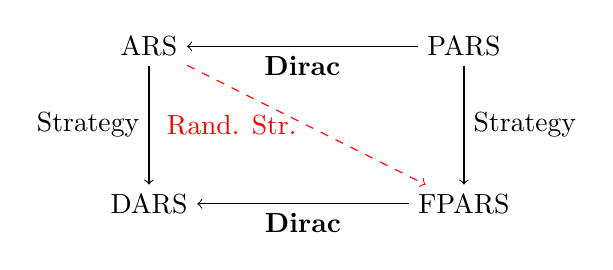
\begin{tikzpicture}
	[node distance=20mm, auto, transform shape]
	\node (m) at (0,0) {ARS};
	\node (n) at (4,0) {PARS};
	\node (l) at (0,-2) {DARS};
	\node (p) at (4,-2) {FPARS};
	\draw (n) edge[->] node[below] {$\textbf{Dirac}$} (m);
	\draw (n) edge[->] node[right] {Strategy} (p);
	\draw (p) edge[->] node[below] {$\textbf{Dirac}$} (l);
	\draw (m) edge[->] node[left] {Strategy} (l);
	\draw (m) edge[->,dashed,color=red] node[left] {Rand. Str.} (p);
	\end{tikzpicture}
\end{minipage}}
	\caption{The diagram showing inclusion relations between different types of ARSs.}
	\label{figure:diagars}
\end{figure}
The way we have introduced FPARSs, however, was different. In fact we have built FPARSs on top of ARSs, in that an FPARS transforms the nondeterministic dynamics of an ARS to a probabilistic one. This way FPARSs are obtained from ARSs fixing a \emph{randomised} strategy.
%*****************************************
